\documentclass[11pt]{article}

\usepackage{amsmath}
\usepackage{amssymb}
\usepackage{graphicx}
\usepackage{hyperref}
\usepackage{bm}
\usepackage{dcolumn}
\usepackage{multirow}
\usepackage{listings}
\usepackage{authblk}

\graphicspath{{../images/}}
\DeclareGraphicsExtensions{.eps,.png,.pdf}
\DeclareMathOperator{\sech}{sech}
\newcolumntype{d}[1]{D{.}{.}{#1} }
\lstset{
	basicstyle=\footnotesize\ttfamily,
	frame=single,
	columns=fixed,
	breaklines=true
}

\graphicspath{{../images/}}
\renewcommand{\figurename}{Figure}
\newcommand{\figurenames}{Figures}
%\newcommand{\figname}{Figure}
%\newcommand{\fignames}{Figures}
\newcommand{\figname}{Fig.}
\newcommand{\fignames}{Figs.}
\newcommand{\equationname}{Equation}
\newcommand{\equationnames}{Equations}
%\newcommand{\eqnname}{Equation}
%\newcommand{\eqnnames}{Equations}
\newcommand{\eqnname}{Eq.}
\newcommand{\eqnnames}{Eqs.}


\begin{document}

\title{Sonar Workbench User's Guide}
\author{Thomas J. Deal}
\affil{Naval Undersea Warfare Center, Newport, RI}
\date{\today}
\maketitle

\begin{abstract}
Abstract goes here.
\end{abstract}

\newpage
\tableofcontents
%\newpage
%\listoftables
%\listoffigures

\newpage
\section{Introduction}\label{sec:intro}
Sonar Workbench is a suite of Matlab tools for the design and analysis of sonar systems. Much of the content is adapted from \emph{An Introduction to Sonar Systems Engineering} \cite{Ziomek}, which is recommended as a companion resource for the user interested in understanding more of the theory.

\section{Coordinate System and Reference Frames}\label{sec:coord}
Sonar Workbench uses a right-handed, Cartesian coordinate system known as North-East-Down (NED), as shown in \figname~\ref{fig:NED}. In this coordinate system, the first coordinate, $x$, points north, the second coordinate, $y$, points east, and the third coordinate, $z$, points down. Roll, $\gamma$, is rotation about the $x$ axis, pitch, $\theta$, is rotation about the $y$ axis, and yaw, $\psi$, is rotation about the $z$ axis. The NED coordinate system is ideal for underwater applications, because depth is measured downward from the surface, yaw is measured clockwise from north, and pitch is measured relative to the horizontal plane.

\begin{figure}[!ht]
\begin{center}
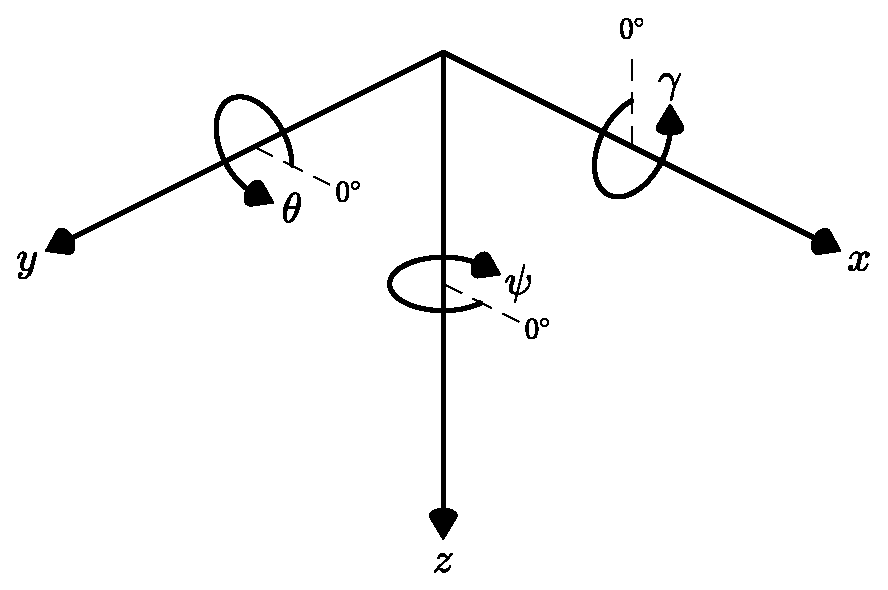
\includegraphics[width=3in]{NEDCoordinateSystem}
\caption{\label{fig:NED}NED coordinate system}
\end{center}
\end{figure}

Sonar Workbench uses three reference frames: the element frame, the array frame, and the body frame. All frames use the NED coordinate system, and each frame can be located relative to another by a combination of translations\footnote{displacement along the $x$, $y$, or $z$ axes} and rotations.

The element frame is always located at the center of the element, with the element's maximum response axis aligned with the $+x$ axis. Exceptions to this alignment are the omnidirectional element, which has no maximum response axis, and the linear element, which the user specifies as initially parallel to one of the three axes ($x$,$y$,$z$) in the element frame. For planar piston elements, the element face lies in the element frame $y$-$z$ plane.

Each element in an array can have arbitrary translation and rotation in the array frame. The array frame origin and orientation is entirely up to the user, but it is typical for planar arrays to be located in center of the array frame's $y$-$z$ plane and for volumetric arrays' geometric center to be located at the origin of the array frame.

The entire array can also be arbitrarily translated and rotated relative to the body frame. For example, a planar array on the nose of a torpedo might have a simple translation along the body frame $x$ axis, while a flank array might have translations along the body $x$ and $y$ axes plus a rotation $\psi$ about the body frame $z$ axis. \figurename~\ref{fig:ReferenceFrames} shows an example of element, array, and body frames for a conformal flank array.

\begin{figure}[!ht]
\begin{center}
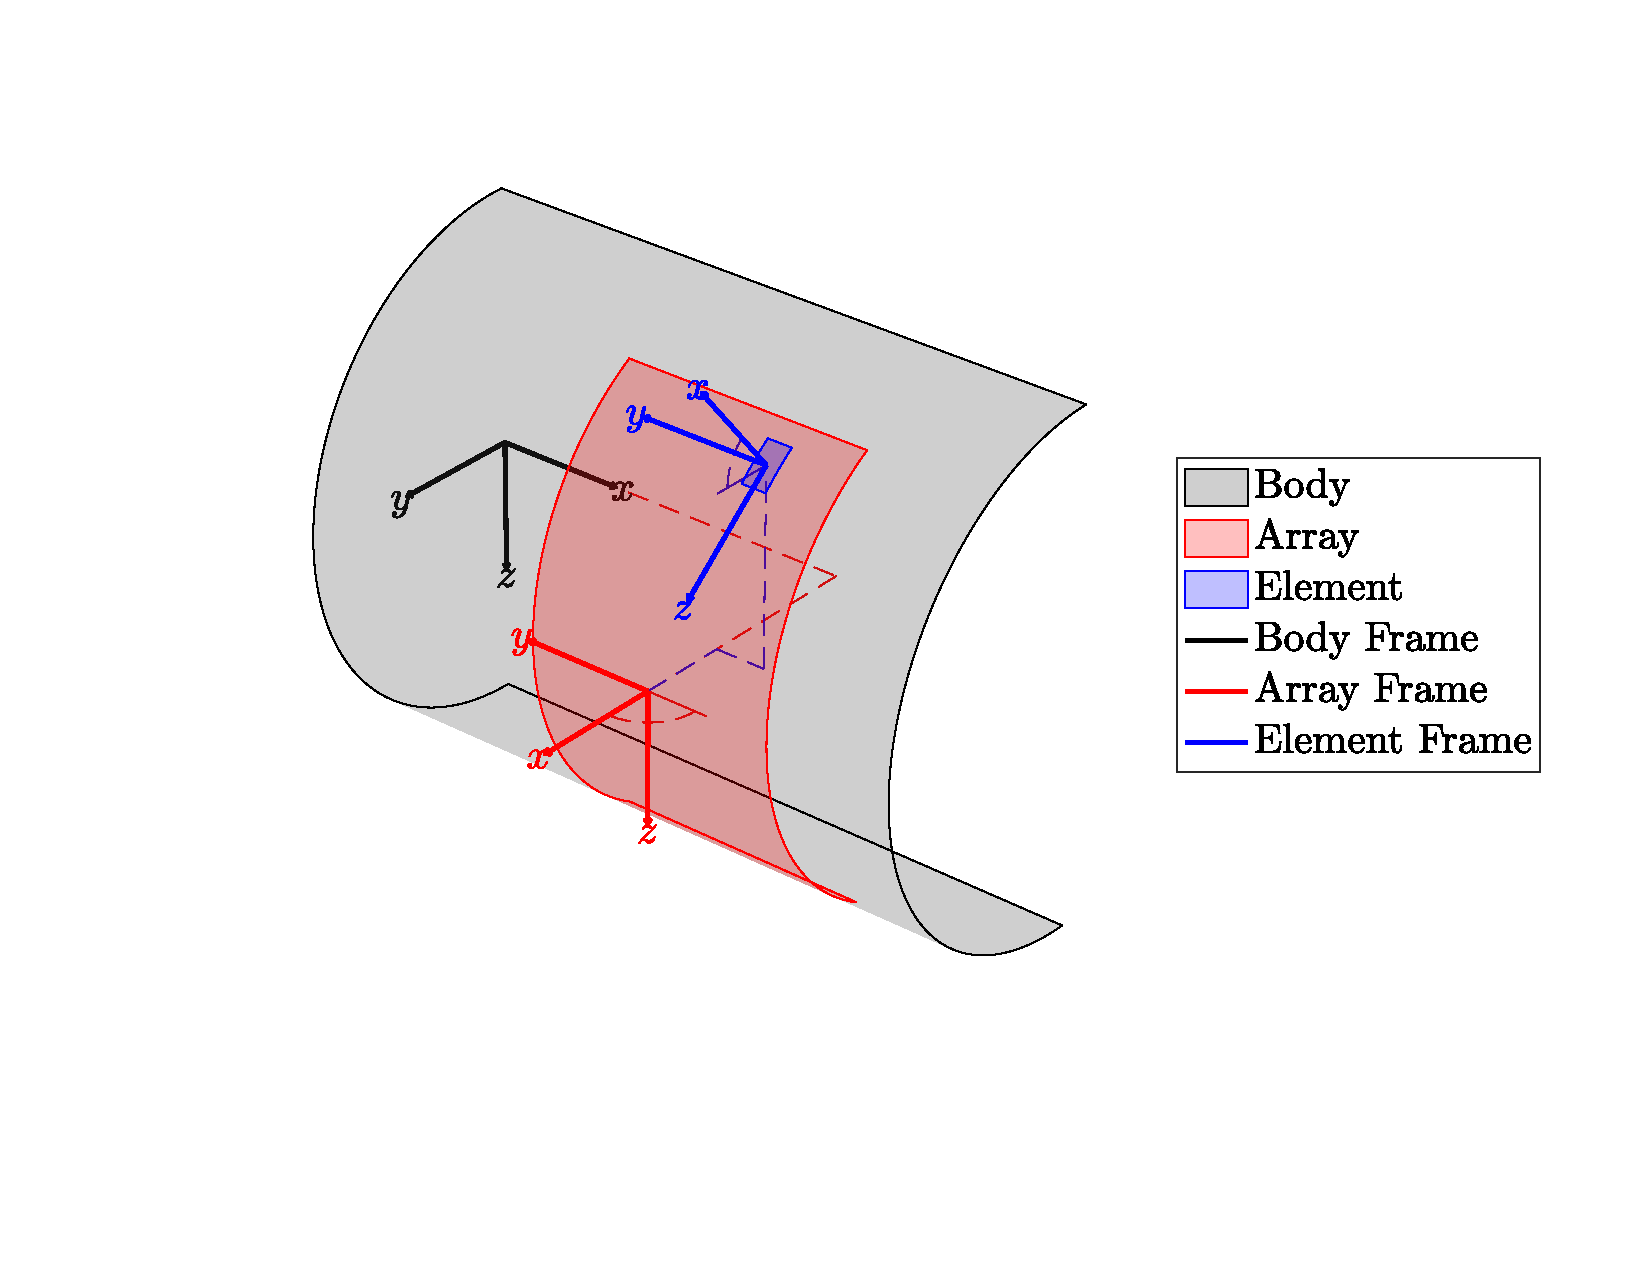
\includegraphics[width=\textwidth]{BodyArrayElementFrame}
\caption{\label{fig:ReferenceFrames}Body, array, and element frames for flank array example}
\end{center}
\end{figure}

Beam patterns are always computed in the body frame as a function of body azimuth angles $\psi$ and elevation angles $\theta$. Azimuth and elevation angles are measured from the body frame $+x$ axis. For simple analyses, the array and body frames can be aligned and colocated to produce beam patterns in the array frame. In this case, beam pattern angles $\psi$ and $\theta$ are measured from the array frame $+x$ axis. More details about element, array, and body frame alignments will be explained in Sections~\ref{sec:element} and \ref{sec:array}.

\section{Elements}\label{sec:element}

Sonar Workbench includes support for the element types listed in Table~\ref{tab:ElementTypes}. It treats each element as a uniformly vibrating surface.

\begin{table}[!ht]
	\begin{center}
		\caption{Supported element types}
		\label{tab:ElementTypes}
		\begin{tabular}{c|l} 
			\textbf{Element Type} & \textbf{Type String} \\
			\hline
			Omnidirectional  & \texttt{`OmnidirectionalElement'} \\
			Uniform Line & \texttt{`LinearElement'} \\
			Cosine & \texttt{`CosineElement'} \\
			Circular Piston & \texttt{`CircularPistonElement'} \\
			Rectangular Piston & \texttt{`RectangulerPistonElement'} \\
			Annular Piston & \texttt{`AnnularPistonElement'} \\
			Hexagonal Piston & \texttt{`HexagonalPistonElement'} \\
		\end{tabular}
	\end{center}
\end{table}

An element structure holds the parameters that define the element. The element structure must contain the \texttt{.type} field with a string corresponding to a \texttt{.m} file that generates the corresponding element pattern. Table~\ref{tab:ElementTypes} lists the built-in element type strings, but the user can easily define additional element types by generating their own element pattern generator script with the same interface. The element \texttt{.baffle} dictates whether the element should be baffled by the element frame $y$-$z$ plane (e.g. arrays mounted to platforms) or unbaffled (e.g. towed arrays, sonobuoys). For visualization purposes, fields \texttt{.shapex}, \texttt{.shapey}, and \texttt{shapez} contain vectors of element shape coordinates. The script \texttt{AddElementShape.m} generates these vectors for the element types listed in Table~\ref{tab:ElementTypes}. The other fields in the element structure depend on the element type, as listed in Table~\ref{tab:ElementFields}.

\begin{table}[!ht]
	\begin{center}
		\caption{Element structure fields}
		\label{tab:ElementFields}
		\begin{tabular}{c|c|l} 
			\textbf{Element Type} & \textbf{Field} & \textbf{Description} \\
			\hline
			\multirow{2}{*}{Uniform Line} & \texttt{.L} & length (m) \\
			& \texttt{.axis} & aligned axis \texttt{`x'}, \texttt{`y'}, \texttt{`z'} \\
			\hline
			Circular Piston & \texttt{.a} & radius (m) \\
			\hline
			\multirow{2}{*}{Rectangular Piston} & \texttt{.w} & width (m) \\
			& \texttt{.h} & height (m) \\
			\hline
			\multirow{2}{*}{Annular Piston} & \texttt{.a} & outer radius (m) \\
			& \texttt{.b} & inner radius (m) \\
			\hline
			Hexagonal Piston & \texttt{.a} & inscribed circle radius (m) \\	
		\end{tabular}
	\end{center}
\end{table}


\section{Arrays}\label{sec:array}

\section{Beams}\label{sec:beam}


\newpage
\bibliographystyle{ieeetr}
\bibliography{SonarWorkbench}

\end{document}